\documentclass[12pt,a4paper]{report}

% ─── Packages ────────────────────────────────────────────────────────────────
\usepackage[top=1in, bottom=1in, left=1.5in, right=1in]{geometry}
\usepackage{graphicx}
\usepackage{setspace}
\usepackage{titlesec}
\usepackage{fancyhdr}
\usepackage{hyperref}
\usepackage{array}
\usepackage{booktabs}
\usepackage{longtable}
\usepackage{enumitem}
\usepackage{parskip}
\usepackage{microtype}
\usepackage{caption}
\usepackage{float}
\usepackage[T1]{fontenc}
\usepackage[utf8]{inputenc}
\usepackage{lmodern}
\usepackage{tocloft}

% ─── Typography ───────────────────────────────────────────────────────────────
\setlength{\parindent}{0ex}
\setlength{\parskip}{5pt}
\renewcommand{\baselinestretch}{1.5}

% ─── Chapter / Section Style ─────────────────────────────────────────────────
\titleformat{\chapter}[block]
  {\normalfont\Large\bfseries\centering}
  {CHAPTER \thechapter:}{0.5em}{\MakeUppercase}
\titlespacing*{\chapter}{0pt}{-10pt}{18pt}

\titleformat{\section}{\normalfont\large\bfseries}{\thesection}{1em}{}
\titleformat{\subsection}{\normalfont\normalsize\bfseries}{\thesubsection}{1em}{}

% ─── Header / Footer — NO running head line ───────────────────────────────────
\pagestyle{fancy}
\fancyhf{}
\fancyfoot[C]{\thepage}
\renewcommand{\headrulewidth}{0pt}

% ─── Hyperref ────────────────────────────────────────────────────────────────
\hypersetup{colorlinks=true, linkcolor=black, urlcolor=blue, citecolor=black}

% ════════════════════════════════════════════════════════════════════════════
\begin{document}
\pagenumbering{roman}

% ─────────────────────────────────────────────────────────────────────────────
%  PAGE 1 — ALL-CAPS COVER  (tu-logo.png)
% ─────────────────────────────────────────────────────────────────────────────
\begin{titlepage}
\thispagestyle{empty}
\setstretch{1.5}
\begin{center}

\includegraphics[height=1.2in,width=1.2in]{tu-logo.png}\\[6pt]

TRIBHUVAN UNIVERSITY\\
INSTITUTE OF SCIENCE AND TECHNOLOGY\\
\textbf{SAMRIDDHI COLLEGE}\\
LOKANTHALI-1, BHAKTAPUR\\[18pt]

INTERNSHIP REPORT\\
ON\\[4pt]
\textbf{FRONTEND DEVELOPMENT}\\
AT\\
CS SEWA PVT. LTD.\\[18pt]

\textbf{SUBMITTED TO:}\\
DEPARTMENT OF COMPUTER SCIENCE AND INFORMATION TECHNOLOGY\\
SAMRIDDHI COLLEGE\\[12pt]

IN PARTIAL FULFILLMENT OF THE REQUIREMENTS FOR THE DEGREE OF\\
BACHELOR OF SCIENCE IN\\
COMPUTER SCIENCE AND INFORMATION TECHNOLOGY\\[18pt]

\textbf{SUBMITTED BY:}\\
\textbf{ANJU ADHIKARI}\\
TU EXAM ROLL NO.: 29279/078\\
TU REGISTRATION NO.: 5-2-1113-91-2021\\[12pt]

MARCH, 2026
\end{center}
\end{titlepage}

% ─────────────────────────────────────────────────────────────────────────────
%  PAGE 2 — MIXED-CASE COVER  (samriddhilogo.png)
% ─────────────────────────────────────────────────────────────────────────────
\newpage
\thispagestyle{empty}
\setstretch{1.5}
\begin{center}

\includegraphics[height=1.2in,width=1.2in]{samriddhilogo.png}\\[6pt]

Tribhuvan University\\
Institute of Science and Technology\\
\textbf{Samriddhi College}\\
Lokanthali-1, Bhaktapur\\[18pt]

Internship Report\\
on\\[4pt]
\textbf{Frontend Development}\\
at\\
\textbf{CS Sewa Pvt. Ltd.}\\[18pt]

\textbf{Submitted to:}\\
Department of Computer Science and Information Technology\\
Samriddhi College\\[12pt]

In partial fulfillment of the requirements for the degree of\\
\textbf{Bachelor of Science in}\\
\textbf{Computer Science and Information Technology}\\[18pt]

\textbf{Submitted by:}\\
\textbf{Anju Adhikari}\\
TU Exam Roll No.: 29279/078\\
TU Registration No.: 5-2-1113-91-2021\\[12pt]

March, 2026
\end{center}

% ─────────────────────────────────────────────────────────────────────────────
%  MENTOR'S RECOMMENDATION
% ─────────────────────────────────────────────────────────────────────────────
\newpage
\thispagestyle{empty}
\setstretch{1.5}
\chapter*{Mentor's Recommendation}

I hereby recommend that this report prepared under my mentorship by
\textbf{Ms.\ Anju Adhikari} entitled \textbf{``Frontend Development at CS Sewa Pvt.\ Ltd.''}
in partial fulfillment of the requirements for the degree of Bachelor of Science in Computer
Science \& Information Technology of Tribhuvan University be processed for review.

\vspace{2.5cm}
\noindent\rule{5cm}{0.4pt}\\[4pt]
\textbf{Er.\ Shree Krishna Khanal}\\
Chief Technical Officer, Internship Mentor\\
CS Sewa Pvt.\ Ltd.\\[8pt]
Date:

% ─────────────────────────────────────────────────────────────────────────────
%  SUPERVISOR'S RECOMMENDATION  (samriddhihead.jpg)
% ─────────────────────────────────────────────────────────────────────────────
\newpage
\thispagestyle{empty}
\setstretch{1.5}
\begin{center}

\includegraphics[scale=0.1]{samriddhihead.jpg}
\end{center}
\begin{center}\large\textbf{Supervisor's Recommendation}\end{center}

I hereby recommend that this internship report entitled \textbf{``Frontend Development at CS
Sewa Pvt.\ Ltd.''} prepared under my supervision by \textbf{Ms.\ Anju Adhikari} in partial
fulfillment of the requirements for the degree of Bachelor of Science in Computer Science \&
Information Technology of Tribhuvan University be processed for review.

\vspace{2.5cm}
\noindent\rule{5cm}{0.4pt}\\[4pt]
\textbf{Mr.\ Abhisek Dewan}\\
Program Coordinator\\
Department of CSIT\\
Samriddhi College\\[8pt]
Date:

% ─────────────────────────────────────────────────────────────────────────────
%  LETTER OF APPROVAL  (samriddhihead.jpg)
% ─────────────────────────────────────────────────────────────────────────────
\newpage
\thispagestyle{empty}
\setstretch{1.5}
\begin{center}

\includegraphics[scale=0.1]{samriddhihead.jpg}
\end{center}
\begin{center}\Large\textbf{Letter of Approval}\end{center}

This is to certify that this internship report prepared by \textbf{Anju Adhikari} entitled
\textbf{``Frontend Development at CS Sewa Pvt.\ Ltd.''} in partial fulfillment of the
requirements for the degree of Bachelor of Science in Computer Science \& Information
Technology has been well studied. In our opinion, it is satisfactory in scope and quality as
a project for the required degree.

\vspace{0.8cm}
\begin{center}\textbf{Evaluation Committee}\end{center}

\vspace{0.3cm}
\begin{center}
\begin{tabular}{p{6cm} p{1.5cm} p{6cm}}
 & & \\[1.8cm]
\rule{5.5cm}{0.4pt} & & \rule{5.5cm}{0.4pt}\\[2pt]
Mr.\ Abhisek Dewan       & & Er.\ Shree Krishna Khanal\\
(Internship Supervisor)  & & (Internship Mentor)\\[2cm]
\rule{5.5cm}{0.4pt} & & \rule{5.5cm}{0.4pt}\\[2pt]
External Examiner        & & Mr.\ Sandeep Shrestha\\
(External Examiner)      & & (Principal)\\
\end{tabular}
\end{center}
\vfill
\noindent Date: \textbf{2082-11-27 BS}

% ─────────────────────────────────────────────────────────────────────────────
%  DECLARATION
% ─────────────────────────────────────────────────────────────────────────────
\newpage
\thispagestyle{empty}
\setstretch{1.5}
\chapter*{Declaration}
\addcontentsline{toc}{chapter}{Declaration}

I hereby declare that this report entitled \textbf{``Frontend Development''} at
\textbf{``CS Sewa Pvt.\ Ltd.''} submitted to the Department of Computer Science \&
Information Technology, Samriddhi College is my original work. I am the only author of
this work and no sources other than those listed here have been used. This work has been
carried out in partial fulfillment of the requirements of the Bachelor's Degree in Computer
Science \& Information Technology (B.Sc.\ CSIT) under the guidance of
\textbf{Mr.\ Abhisek Dewan}.

\vspace{2.5cm}
\noindent\rule{5cm}{0.4pt}\\[4pt]
\textbf{Anju Adhikari}\\
TU Exam Roll No.: 29279/078\\
TU Registration No.: 5-2-1113-91-2021

% ─────────────────────────────────────────────────────────────────────────────
%  ACKNOWLEDGEMENTS
% ─────────────────────────────────────────────────────────────────────────────
\newpage
\chapter*{Acknowledgements}
\addcontentsline{toc}{chapter}{Acknowledgements}

This internship at CS Sewa Pvt.\ Ltd.\ in the field of Frontend Development has been a
truly rewarding experience, and I am deeply grateful to the many individuals who
contributed to my growth during this period.

I extend my sincere gratitude to the entire team at CS Sewa Pvt.\ Ltd.\ for their warm
welcome and continuous support. I am particularly indebted to my mentor,
\textbf{Er.\ Shree Krishna Khanal}, Chief Technical Officer, whose guidance and technical
mentorship were invaluable throughout the internship.

I would also like to thank the faculty and staff of Samriddhi College. I am especially grateful
to my supervisor, \textbf{Mr.\ Abhisek Dewan}, for his constant encouragement, constructive
feedback, and patience, which were instrumental in shaping this report into its final form.

Finally, I express my deepest gratitude to my family and friends for their constant moral
support throughout my academic journey.

\vspace{0.5cm}
\noindent\textbf{Anju Adhikari}\\
B.Sc.\ CSIT, 8th Semester, Samriddhi College

% ─────────────────────────────────────────────────────────────────────────────
%  ABSTRACT
% ─────────────────────────────────────────────────────────────────────────────
\newpage
\chapter*{Abstract}
\addcontentsline{toc}{chapter}{Abstract}

This report presents the work undertaken during a three-month internship at CS Sewa
Pvt.\ Ltd., an enterprise software development company in Koteshwor, Kathmandu, Nepal.
The internship focused on the frontend development of the \textbf{Agriculture Management
System (AMS)}, a web-based platform for digitizing agricultural data management across
Nepali municipalities.

The primary technologies used were React.js 18 with TypeScript, Ant Design, Axios, and
React Router v6, integrated with a Java Spring Boot backend via JWT-secured REST APIs.
Key areas of work included API integration and testing with Postman, role-based access
control (RBAC), bilingual (Nepali/English) UI/UX design, cascading Nepal address
hierarchy, Leaflet.js map integration for land plot visualization, and deployment of the
production frontend to a government cloud server using WinSCP and PuTTY. Public-facing
pages for notices, downloads, FAQs, weather, and NARC soil analysis were also developed.

The internship provided comprehensive exposure to professional agile development
practices, API-first development workflows, and the unique localization requirements of
Nepal's government IT sector.

\textbf{Keywords}--- Agriculture Management System, React.js, TypeScript, API testing,
Postman, JWT, RBAC, WinSCP, PuTTY, Ant Design, Leaflet, Nepal municipalities

% ─────────────────────────────────────────────────────────────────────────────
%  TOC / LISTS
% ─────────────────────────────────────────────────────────────────────────────
\newpage
\tableofcontents
\newpage
\listoffigures
\newpage
\listoftables

% ─────────────────────────────────────────────────────────────────────────────
%  ABBREVIATIONS
% ─────────────────────────────────────────────────────────────────────────────
\newpage
\chapter*{List of Abbreviations}
\addcontentsline{toc}{chapter}{List of Abbreviations}

\begin{longtable}{p{3cm} p{10cm}}
\textbf{AMS}  & Agriculture Management System \\
\textbf{API}  & Application Programming Interface \\
\textbf{CORS} & Cross-Origin Resource Sharing \\
\textbf{CRUD} & Create, Read, Update, Delete \\
\textbf{DTO}  & Data Transfer Object \\
\textbf{GIS}  & Geographic Information System \\
\textbf{HTTP} & HyperText Transfer Protocol \\
\textbf{IT}   & Information Technology \\
\textbf{JWT}  & JSON Web Token \\
\textbf{NARC} & Nepal Agricultural Research Council \\
\textbf{RBAC} & Role-Based Access Control \\
\textbf{REST} & Representational State Transfer \\
\textbf{SCP}  & Secure Copy Protocol \\
\textbf{SPA}  & Single Page Application \\
\textbf{SSH}  & Secure Shell \\
\textbf{TU}   & Tribhuvan University \\
\textbf{UI}   & User Interface \\
\textbf{UX}   & User Experience \\
\textbf{URL}  & Uniform Resource Locator \\
\end{longtable}

% ════════════════════════════════════════════════════════════════════════════
%  CHAPTER 1: INTRODUCTION
% ════════════════════════════════════════════════════════════════════════════
\newpage
\pagenumbering{arabic}

\chapter{Introduction}

\section{Introduction}

Frontend development is a central pillar of modern software engineering, bridging complex
backend systems and the end users who rely on them daily. In Nepal's rapidly growing
government IT sector, the quality of a web application's interface directly determines its
adoption, especially when it must serve Nepali-speaking users who depend on localized
interfaces for all official records (Adhikari et al., 2022).

Agriculture contributes significantly to Nepal's GDP and employs the majority of its
rural workforce. Yet municipal agricultural data management remains largely paper-based,
causing delays, inaccuracies, and administrative inefficiency. The push for digital
governance has created demand for well-designed web platforms that are bilingual,
locally relevant, and connected to secure, testable backend APIs (Food and Agriculture
Organization of the United Nations [FAO], 2021).

CS Sewa Pvt.\ Ltd.\ is a Kathmandu-based enterprise software company specializing in
government and municipal web applications. The internship here focused on the
\textbf{Agriculture Management System (AMS)}, a production system serving multiple
Nepali municipalities. The work covered API integration and testing, role-based access
control, bilingual UI/UX design, Nepal-specific localization, and deployment of the
production frontend to a government cloud server using WinSCP and PuTTY
(Banks \& Porcello, 2020).

\section{Problem Statements}

Municipal agricultural offices lack a unified digital system. Manual data entry for farmer
records, land plots, subsidies, and production data leads to inconsistencies and delays.
Existing generic tools are not adapted for Nepali language interfaces or multi-municipality
support. Without role-based access control, data security and departmental boundaries
cannot be enforced (Ferraiolo et al., 2001).

\section{Objectives}

The Agriculture Management System aims to digitize and centralize agricultural data management
for Nepali municipalities by replacing traditional paper-based processes with a secure and
accessible web platform. The specific objectives of the project are:

\begin{itemize}

\item To develop a digital platform for managing farmer records, land plots, subsidies,
      and agricultural production data.

\item To implement role-based access control to ensure secure and organized access
      for different users such as executives, officers, and farmers.

\item To provide a bilingual interface (Nepali and English) to support local users
      and improve system accessibility.

\item To enable visualization and management of agricultural land through an
      interactive map-based module.

\end{itemize}

\section{Scope and Limitations}

The scope covers complete frontend development and deployment of the AMS for municipalities including Chandannath, Swamikartik, Patarasi, and Budhiganga. All API communication is authenticated using JWT Bearer tokens and tested through Postman. Deployment includes Vite production builds, secure file transfer using WinSCP, and Nginx configuration via PuTTY.

Limitations include the absence of offline data entry support for areas with poor connectivity. The system does not provide real-time multi-user synchronization. Advanced analytics dashboards were deferred beyond the internship period.

\section{Report Organization}

Chapter 2 covers the organization and literature review. Chapter 3 explains internship activities, project details, and tasks performed. Chapter 4 presents the conclusions and learning outcomes.

% ════════════════════════════════════════════════════════════════════════════
%  CHAPTER 2: ORGANIZATION AND LITERATURE REVIEW
% ════════════════════════════════════════════════════════════════════════════
\chapter{Organization Details and Literature Review}

\section{Introduction to Organization}

CS Sewa Pvt.\ Ltd.\ (Creative Solution Sewa Private Limited) is an enterprise software
development company in Koteshwor, Kathmandu, Nepal. It delivers full-stack web
applications for government agencies, municipalities, and private sector clients across
Nepal, with a focus on agricultural management, building permit systems, and municipal
governance platforms (CS Sewa Pvt. Ltd., 2024).

\begin{table}[H]
\centering
\caption{Organizational Details of CS Sewa Pvt. Ltd.}
\renewcommand{\arraystretch}{1.4}
\begin{tabular}{|p{5.5cm}|p{7.5cm}|}
\hline
\textbf{Organization Name} & Creative Solution Sewa Pvt. Ltd. \\
\hline
\textbf{Location} & Koteshwor, Kathmandu, Nepal \\
\hline
\textbf{Opening Hours} & 10:00 AM to 6:00 PM \\
\hline
\textbf{Contact} & +977-9745335854 \\
\hline
\textbf{Email} & cssewanepal@gmail.com \\
\hline
\textbf{Website} & www.cssewa.com.np \\
\hline
\end{tabular}
\end{table}

\section{Organizational Hierarchy}

The company is led by the Board of Directors and CEO, under whom a Technical Project
Manager, Administrative Manager, and Operation Manager operate in parallel. The
Technical Project Manager supervises the Software Development and Quality Assurance
teams, structured into Backend, Frontend, and Mobile sub-teams.

\begin{figure}[H]
\centering
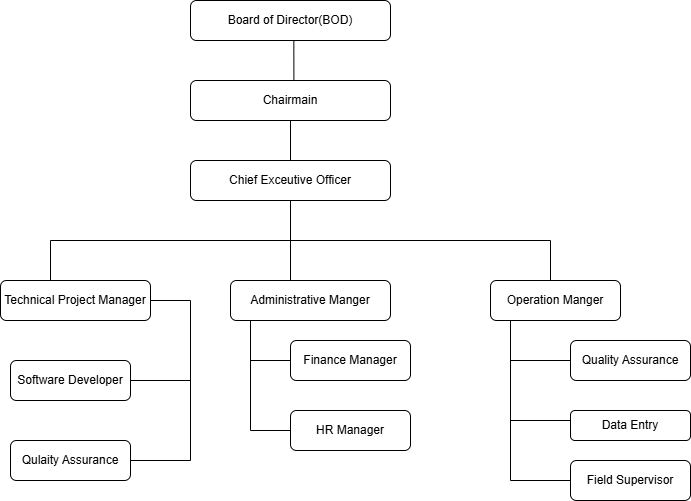
\includegraphics[width=0.82\textwidth]{officeHeirarchy.png}
\caption{Organizational Hierarchy of CS Sewa Pvt. Ltd.}
\label{fig:org_hierarchy}
\end{figure}

\section{Working Domains of Organization}

\textbf{Government IT Solutions:} Agricultural management portals, building permit
systems, and municipal data platforms for local governments across Nepal.

\textbf{Enterprise Application Development:} Full-stack systems for universities, schools,
hospitals, and private sector organizations with complex workflows.

\textbf{Field Data Collection:} Structured field surveys and data collection with integrated
digital management systems for municipalities.

\textbf{System Integration and Database Management:} Secure data migration, API
integration, and legacy system modernization services.

\section{Description of Intern Department/Unit}

The internship was carried out within the \textbf{Web Development Department}, which
builds full-stack applications using Java Spring Boot (backend) and React.js/TypeScript
(frontend) following Ant Design standards. The team works in an Agile/Scrum environment
with weekly sprint cycles, daily stand-ups, and code reviews.

\begin{table}[H]
\centering
\caption{Internship Details}
\renewcommand{\arraystretch}{1.4}
\begin{tabular}{|p{5.5cm}|p{7.5cm}|}
\hline
\textbf{Start Date} & November 15, 2025 \\
\hline
\textbf{End Date} & February 15, 2026 \\
\hline
\textbf{Duration} & 3 Months \\
\hline
\textbf{Days of Work} & Sunday to Friday (6 Days) \\
\hline
\textbf{Working Hours} & 10:00 AM to 6:00 PM \\
\hline
\end{tabular}
\end{table}

\section{Literature Review}

\subsection{Digital Agriculture Management Systems}

The transition from paper-based to digital agricultural data management has been a
priority in both developed and developing countries seeking to improve the accuracy and
efficiency of municipal agricultural governance. The Food and Agriculture Organization
of the United Nations (2021) reviewed digital agriculture initiatives across Asia and
Africa and found that web-based platforms that consolidate farmer registries, land
records, subsidy programs, and production data into a single system significantly reduce
administrative overhead and improve subsidy distribution accuracy at the local government
level. The FAO report specifically identifies the lack of integration between farmer
identity records, land ownership data, and subsidy disbursement as the primary source
of inefficiency in municipal agricultural offices — exactly the problem the Agriculture
Management System developed during this internship is designed to address by providing
unified CRUD modules for each of these data domains within a single authenticated
platform.

Adhikari et al.\ (2022) examined the practical challenges of building government web
applications for Nepal's municipal sector and found that the absence of digitized
agricultural data management forces field officers to maintain parallel paper and digital
records, leading to data inconsistencies and delays in subsidy processing. Their study
of multiple Nepali municipality IT deployments concluded that systems designed with
Nepal-specific localization — including Devanagari-language interfaces and cascading
Province--District--Municipality--Ward address hierarchies — achieve significantly
higher adoption rates among municipal staff than generic international platforms, because
staff can navigate and enter data in their primary working language without translation
overhead.

\subsection{Role-Based Access Control in Government Web Platforms}

Government agricultural management systems typically serve multiple user categories
with distinct data access requirements — from field-level data entry officers to
executive decision-makers and system administrators. Ferraiolo et al.\ (2001) proposed
and formalized the NIST standard for Role-Based Access Control (RBAC), demonstrating
that enforcing access boundaries based on organizational roles is more scalable and
auditable than individual-level permission management in multi-user government systems.
Their framework, which separates role assignment, role authorization, and permission
authorization, directly maps to the five-role architecture of the AMS — Superadmin,
Executive, Revenue, Department, and Farmer — where each role is assigned a distinct
set of module access permissions enforced at both the route and UI rendering levels.

Jones et al.\ (2015) established JSON Web Token (JWT) as the standard mechanism for
carrying role claims in stateless REST API authentication, enabling the frontend to
decode the user's role from the token payload and enforce UI-level access control
without an additional API call on every navigation event. This approach is particularly
well suited to single-page applications serving multiple roles, as it allows the React
Router private route wrappers and conditional sidebar rendering in the AMS to make
authorization decisions entirely on the client side once the token has been validated.

\subsection{React.js and TypeScript for Government Web Applications}

Banks and Porcello (2020) conducted a comprehensive study of React.js patterns for
production-scale single-page applications and found that the component-based
architecture, combined with React's unidirectional data flow, is particularly well suited
to government data management platforms that require consistent UI patterns across a
large number of CRUD modules. Their analysis of large-scale React deployments showed
that centralizing shared state — such as authentication context and language preferences
— in React Context providers, rather than duplicating it across components, significantly
reduces maintenance cost as the application grows. This pattern is directly reflected in
the AMS architecture, where a single \texttt{LanguageContext} and a centralized Axios
instance with JWT interceptors serve all modules uniformly.

Cherny (2019) demonstrated that adopting TypeScript's static type system in React
applications significantly reduces the frequency of runtime integration errors caused by
API contract mismatches between frontend and backend teams. In a multi-module
government system like the AMS — where each module consumes a different set of
Spring Boot REST API endpoints — TypeScript interfaces derived from the backend DTO
schemas provide compile-time guarantees that request payloads and response structures
are correctly typed before any code reaches production.

\subsection{REST API Integration and Testing Practices}

Sohan et al.\ (2017) studied the role of API documentation and structured testing in
reducing integration defects in web development teams and found that developers who
tested API endpoints systematically using organized collections — with environment
variables for base URLs and authentication tokens, and explicit test cases for success,
authentication failure, authorization failure, and validation error scenarios — detected
integration issues significantly earlier in the development cycle compared to teams that
tested APIs only implicitly during frontend development. This finding directly motivated
the Postman-first workflow adopted throughout the AMS internship, where a dedicated
Postman collection was built and fully validated for each module before any frontend
component was written, ensuring that TypeScript interfaces and error-handling logic
were based on verified API behaviour rather than assumptions.

% ════════════════════════════════════════════════════════════════════════════
%  CHAPTER 3: INTERNSHIP ACTIVITIES
% ════════════════════════════════════════════════════════════════════════════
\chapter{Internship Activities}

\section{Roles and Responsibilities}

The role during this internship was \textbf{Frontend Developer Intern}, responsible for
designing and implementing React.js/TypeScript components, conducting API testing with
Postman, and collaborating with the backend team on the Agriculture Management System.
Key responsibilities included:

\begin{itemize}
  \item Design and implement bilingual (Nepali/English) React.js/TypeScript components
        for all CRUD modules of the Agriculture Management System.
  \item Test all backend REST API endpoints using Postman: verify request/response
        formats, authentication flows, and error handling before frontend integration.
  \item Integrate all modules with Spring Boot APIs using Axios with JWT interceptors.
  \item Implement role-based route protection (Superadmin, Executive, Revenue, Department, Farmer).
  \item Build Nepal-specific UI components: cascading address dropdowns.
  \item Integrate Leaflet maps for agricultural land plot visualization.
  \item Develop public-facing pages: notices, downloads, FAQ, weather, soil analysis.
  \item Build the production Vite bundle and deploy to the government cloud server
        using WinSCP for file transfer and PuTTY for SSH server administration.
  \item Participate in sprint planning, stand-ups, and code reviews.
  \item Self-test each feature locally before raising pull requests.
\end{itemize}
\newpage
\section{Weekly Log}

\begin{longtable}{|p{2.8cm}|p{11cm}|}
\caption{Weekly Log with Tasks Description} \label{tab:weekly_log} \\
\hline
\textbf{Week} & \textbf{Tasks Performed} \\
\hline
\endfirsthead
\hline
\textbf{Week} & \textbf{Tasks Performed} \\
\hline
\endhead

\textbf{Week 1}
 &
Onboarding; set up dev environment (Node.js, Vite, VS Code, Git);
explored codebase and project architecture; reviewed Ant Design documentation;
studied Spring Boot API structure with Postman. \\
\hline

\textbf{Week 2}
 &
Tested authentication APIs in Postman (login, refresh, logout);
implemented JWT login flow; configured Axios request/response interceptors
for Bearer token and 401 redirect; built base layout with role-aware sidebar. \\
\hline

\textbf{Week 3}
 &
Developed bilingual language context (Nepali/English);
built cascading Province $\to$ District $\to$ Municipality $\to$ Ward dropdowns;
tested address hierarchy APIs in Postman. \\
\hline

\textbf{Week 4}
 &
Tested farmer CRUD APIs (GET, POST, PUT, DELETE) in Postman;
built Farmer Registration multi-step form with photo upload;
implemented farmer list with search, filter, and pagination;
integrated APIs with full error handling. \\
\hline

\textbf{Week 5}
 &
Tested land plot and GeoJSON APIs in Postman;
developed Land Plot module with react-leaflet map;
implemented polygon drawing for boundary marking;
built land list filtered by ward and land type; fixed CORS issue. \\
\hline

\textbf{Week 6}
 &
Tested subsidy program and disbursement APIs in Postman;
built Subsidy Management module with program list and application tracking;
implemented multi-municipality config pattern;
applied dynamic form fields per subsidy type. \\
\hline

\textbf{Week 7}
 &
Tested agro-production APIs for all crop types/seasons in Postman;
developed Agro-Production Records module with sortable Ant Design tables;
built batch import interface for bulk data upload. \\
\hline

\textbf{Week 8}
 &
Tested energy and financial APIs in Postman;
developed Energy Usage Records module;
built Financial Records module (income, expenditure, transaction history);
created print-ready financial summary view; demo to mentor. \\
\hline

\textbf{Week 9}
 &
Tested household survey APIs (dynamic field endpoints) in Postman;
developed Household Survey module with dynamic form builder;
built survey response list and export feature. \\
\hline

\textbf{Week 10}
 &
Tested public API endpoints (notices, downloads, weather, soil analysis) in Postman;
developed Notice Board and Download Center;
built bilingual FAQ accordion; integrated weather and NARC soil analysis APIs. \\
\hline

\textbf{Week 11}
 &
Cross-browser testing (Chrome, Firefox, Edge);
resolved TypeScript strict mode errors and ESLint warnings;
optimized re-renders with React.memo/useCallback/useMemo;
fixed Vite cache issues; sprint review and retrospective. \\
\hline

\textbf{Week 12}
&
Final end-to-end testing of all modules;
re-tested all API collections in Postman as final integration check;
resolved remaining bugs; built production Vite bundle; deployed frontend to
government cloud server via WinSCP and PuTTY; configured Nginx; verified live deployment. \\
\hline

\end{longtable}

\section{Description of the Project}

The main project during the internship was the \textbf{Agriculture Management System
(AMS)}, a web-based platform digitizing agricultural data for Nepali municipalities
including Chandannath, Swamikartik, Patarasi, and Budhiganga. The frontend is built
with React.js 18 and TypeScript, bundled with Vite, and communicates with a Java
Spring Boot backend via JWT-secured REST APIs.

\subsection{System Overview}

The AMS follows a three-tier architecture as shown in Figure 3.1. The Presentation Layer consists of the React.js frontend serving two distinct user groups: authenticated municipal staff (Superadmin, Executive, Revenue Officer, Department Officer, and Farmer) managing agricultural data, and unauthenticated citizens accessing public information pages. The Application Layer is a Spring Boot REST API that processes all requests, with all API calls made through Axios with JWT Bearer tokens attached via request interceptors. React Router v6 private route wrappers enforce role-based navigation. All APIs were organized into Postman collections and tested per module before frontend development began.

\begin{figure}[H]
\centering
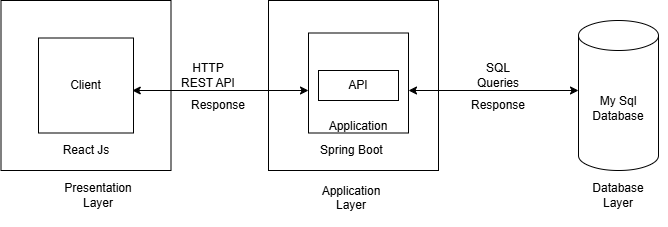
\includegraphics[width=0.82\textwidth]{system_arch.png}
\caption{System Architecture of the Agriculture Management System}
\label{fig:sys_arch}
\end{figure}



\subsection{Architecture of the System}

The AMS follows a three-tier client-server architecture. The React.js/TypeScript SPA
(frontend) communicates exclusively via RESTful HTTP APIs with the Spring Boot
application layer, which in turn manages data persistence via JPA/Hibernate on a
MySQL database. The frontend is bundled by Vite and deployed as a static SPA
on a Linux-based government cloud server behind an Nginx reverse proxy.

\begin{table}[H]
\centering
\caption{Technology Stack}
\renewcommand{\arraystretch}{1.4}
\begin{tabular}{|p{4.2cm}|p{8.8cm}|}
\hline
\textbf{Category} & \textbf{Technology / Tool} \\
\hline
Frontend Framework & React.js 18 with TypeScript \\
\hline
Build Tool & Vite \\
\hline
UI Library & Ant Design (antd) \\
\hline
HTTP Client & Axios \\
\hline
Routing & React Router v6 \\
\hline
Maps & Leaflet.js / react-leaflet \\
\hline
State Management & React Context API \\
\hline
Backend & Java Spring Boot \\
\hline
Authentication & JWT (JSON Web Token) \\
\hline
API Testing & Postman \\
\hline
File Transfer & WinSCP (SFTP/SCP) \\
\hline
Remote Administration & PuTTY (SSH) \\
\hline
Web Server & Nginx \\
\hline
Version Control & Git / GitHub \\
\hline
IDE & Visual Studio Code \\
\hline
\end{tabular}
\end{table}

\section{Tasks and Activities Performed}

\subsection{API Integration and Testing with Postman}

API testing was the first activity performed for each module before writing any frontend
code. Postman collections were created and organized by domain: Authentication, Farmer,
Land Plot, Subsidy, Production, Energy, Financial, Survey, and Public. Environment
variables were configured for the base URL, JWT access tokens, and municipality ID.

For each module, all HTTP methods (GET, POST, PUT, DELETE) were executed and
validated. Request bodies were constructed matching the backend DTO schemas, and
response payloads were inspected to define TypeScript interfaces for type-safe integration.
The following scenarios were tested for every module:

\begin{itemize}
  \item \textbf{Happy path:} correct request returns expected 200/201 response with
        proper payload structure.
  \item \textbf{Authentication:} 401 Unauthorized is returned when the Authorization
        header is missing or token is expired.
  \item \textbf{Authorization:} 403 Forbidden is returned when a lower-privilege role
        attempts a restricted operation.
  \item \textbf{Validation errors:} 400 Bad Request is returned with descriptive
        error messages when required fields are missing or invalid.
  \item \textbf{Not found:} 404 is returned for non-existent resource IDs.
\end{itemize}

This systematic pre-integration testing reduced frontend debugging time significantly
and provided clear API contract documentation for the entire team.

\begin{figure}[H]
\centering
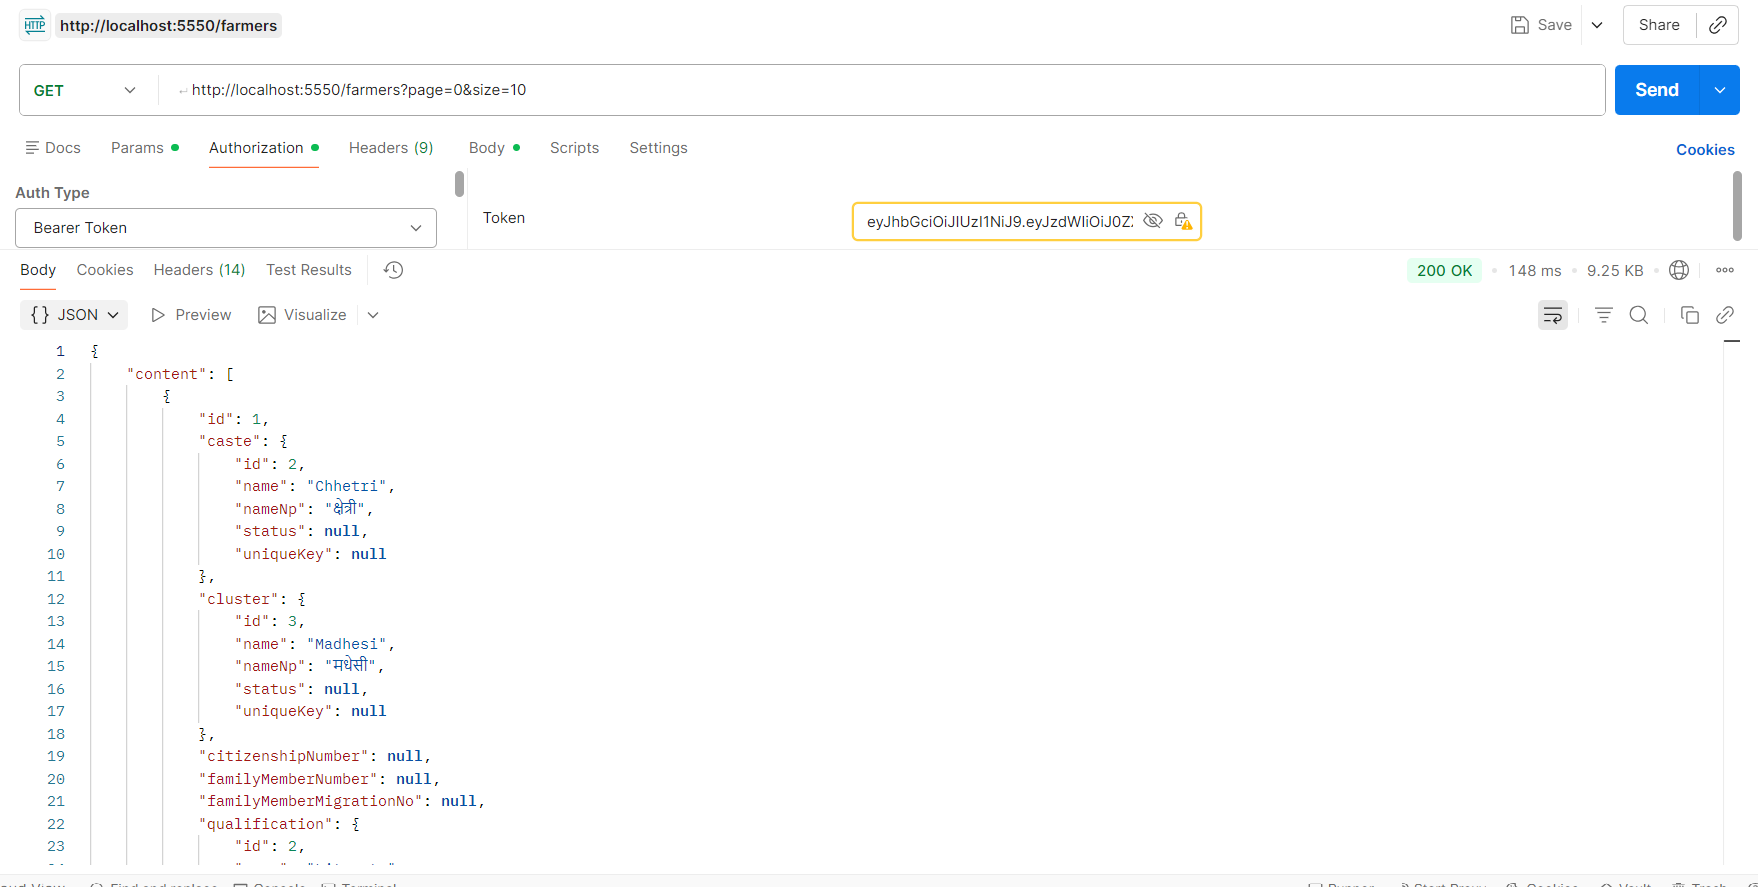
\includegraphics[width=0.85\textwidth]{postman_testing.png}
\caption{Postman API Testing --- Farmer Module Collection}
\label{fig:postman}
\end{figure}

\begin{figure}[H]
\centering
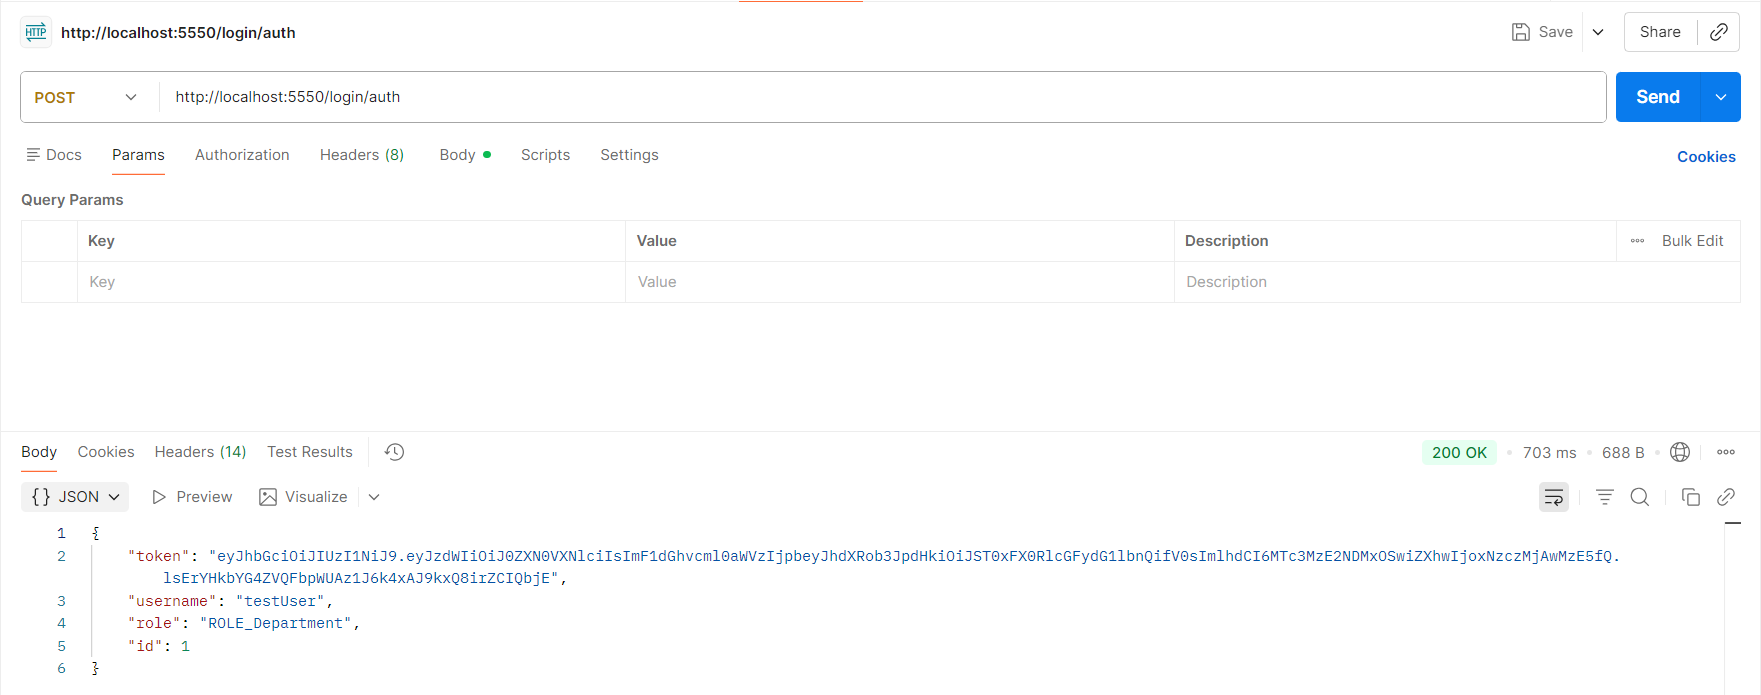
\includegraphics[width=0.85\textwidth]{postman_auth.png}
\caption{Postman API Testing --- Authentication Endpoint (Login)}
\label{fig:postman_auth}
\end{figure}

\subsection{JWT Authentication and Axios Integration}

The authentication flow was implemented as follows. The login page submits credentials
to the Spring Boot auth endpoint. On success, the JWT access token is stored in memory
and managed through an Axios instance with two interceptors:

\begin{itemize}
  \item \textbf{Request interceptor:} automatically attaches the
        \texttt{Authorization: Bearer \{token\}} header to every outgoing API request.
  \item \textbf{Response interceptor:} catches 401 Unauthorized responses, attempts a
        token refresh, and on failure clears the session and redirects to the login page.
\end{itemize}

This ensures all modules share a single, centralized authentication mechanism without
duplicating token-handling logic across components.

\subsection{Role-Based Access Control (RBAC) and UI/UX Design}

Three user roles are supported: \textbf{ROLE\_Superadmin}, \textbf{ROLE\_Executive},
\textbf{ROLE\_Revenue}, \textbf{ROLE\_Department}, and \textbf{ROLE\_Farmer}. RBAC is implemented at two levels in the frontend:

\textbf{Route level:} React Router v6 private route wrappers check the decoded JWT role
claim on every navigation event. Users attempting to access unauthorized routes are
redirected to a 403 page rather than seeing a blank screen or error.

\textbf{UI level:} The sidebar navigation menu is rendered conditionally based on the
active user's role. Action buttons (Create, Edit, Delete, Approve) are shown only to
roles that have permission to perform them, reducing user confusion and preventing
accidental misuse. Ant Design's \texttt{Menu}, \texttt{Button}, and \texttt{Tag}
components are used to visually differentiate role-specific elements.

From a \textbf{UX perspective}, the interface was designed around the following principles:
(i) consistency across all CRUD modules using Ant Design's table-modal pattern;
(ii) clear visual feedback via Ant Design notifications for success, error, and loading
states; (iii) responsive layout supporting both desktop and tablet screen sizes; and
(iv) bilingual support ensuring all labels, messages, and placeholders adapt to the
active language without page reload.

\begin{figure}[H]
\centering
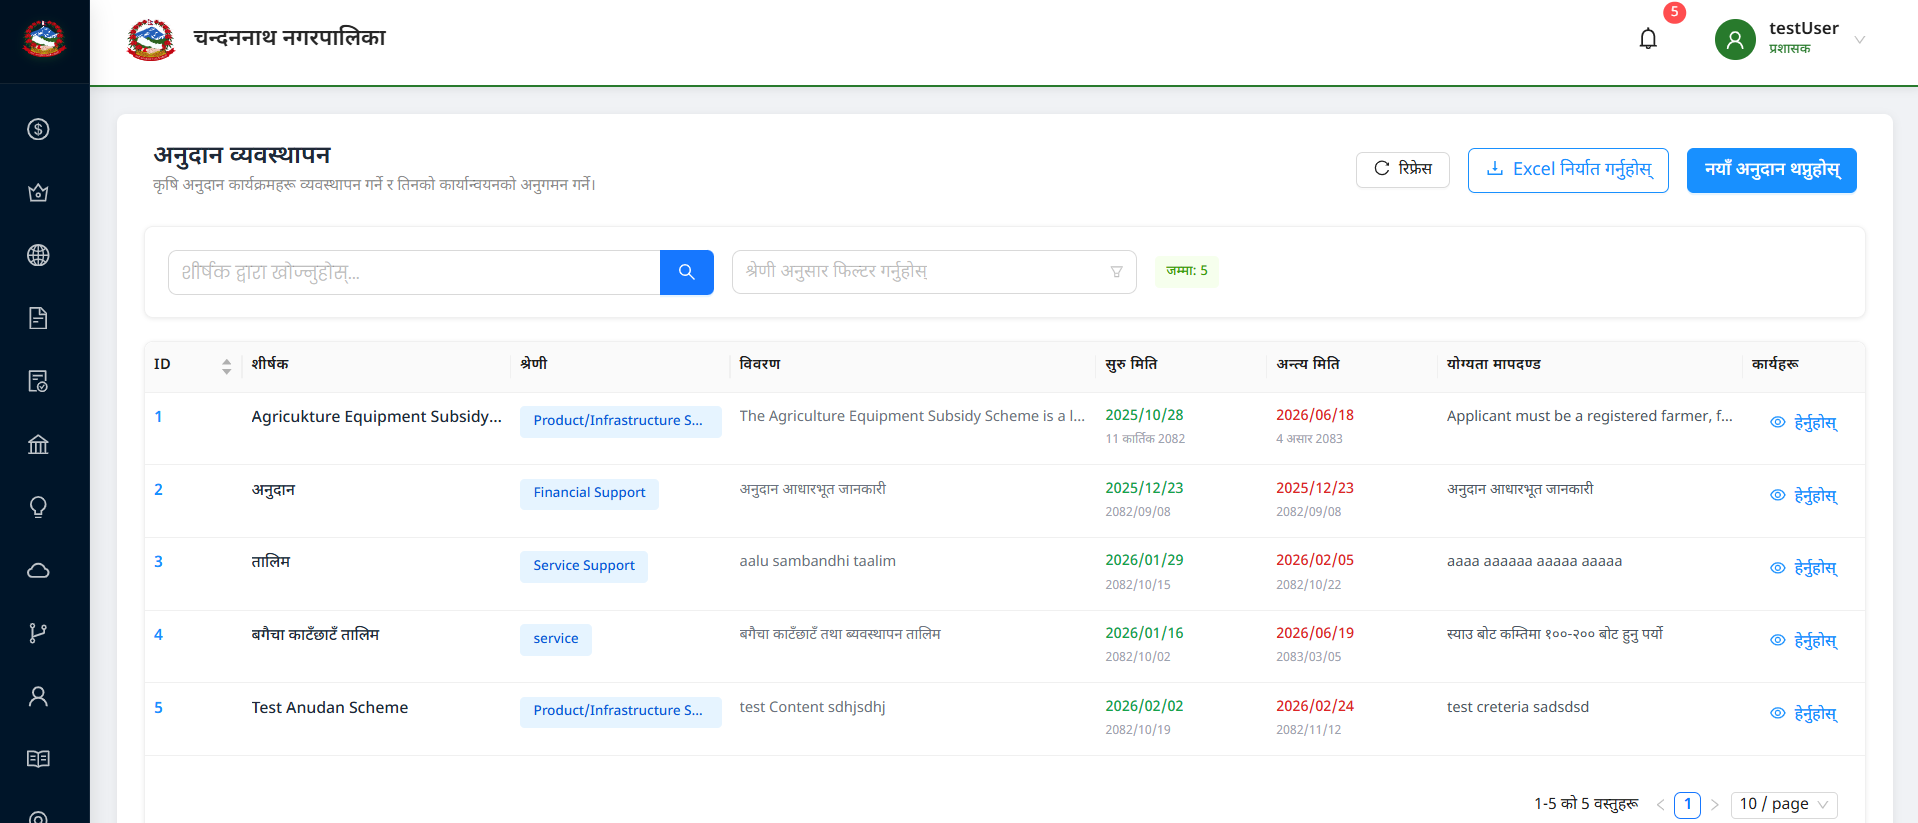
\includegraphics[width=0.85\textwidth]{dashboard.png}
\caption{Admin Dashboard --- Subsidy Management Module (Default Landing View)}
\label{fig:dashboard}
\end{figure}

\subsection{Bilingual UI and Localization}

A \texttt{LanguageContext} was implemented using React Context API, exposing an
\texttt{activeLanguage} state (\texttt{'en'} or \texttt{'ne'}) and a \texttt{toggleLanguage}
function. All UI strings are stored in a structured translations object keyed by language
code. Components consume the context to render the correct text at runtime without
any page reload. This design ensures the bilingual toggle works seamlessly across all
pages, including the public-facing sections accessible without authentication.

\subsection{Cascading Nepal Address Hierarchy}

A reusable \texttt{NepalAddressSelect} component was built for the four-level Nepal
administrative hierarchy: Province $\to$ District $\to$ Municipality $\to$ Ward. Each
level is fetched from the backend API dynamically on selection of the preceding level,
preventing the need to preload the entire address dataset. The component was designed
as a self-contained controlled component with a clean props interface, making it
pluggable across all modules requiring address input.

\subsection{Farmer Management Module}

The Farmer Management module is the primary data entry interface of the AMS. It
features a multi-step Ant Design Form for new farmer registration covering personal
information, address (via the cascading hierarchy component), land ownership details,
crop preferences, and photograph upload. The farmer list view provides server-side
search, multi-criteria filtering, and paginated results. Each farmer's profile page
displays all linked land plots, subsidy history, and production records in tabbed panels.

\begin{figure}[H]
\centering
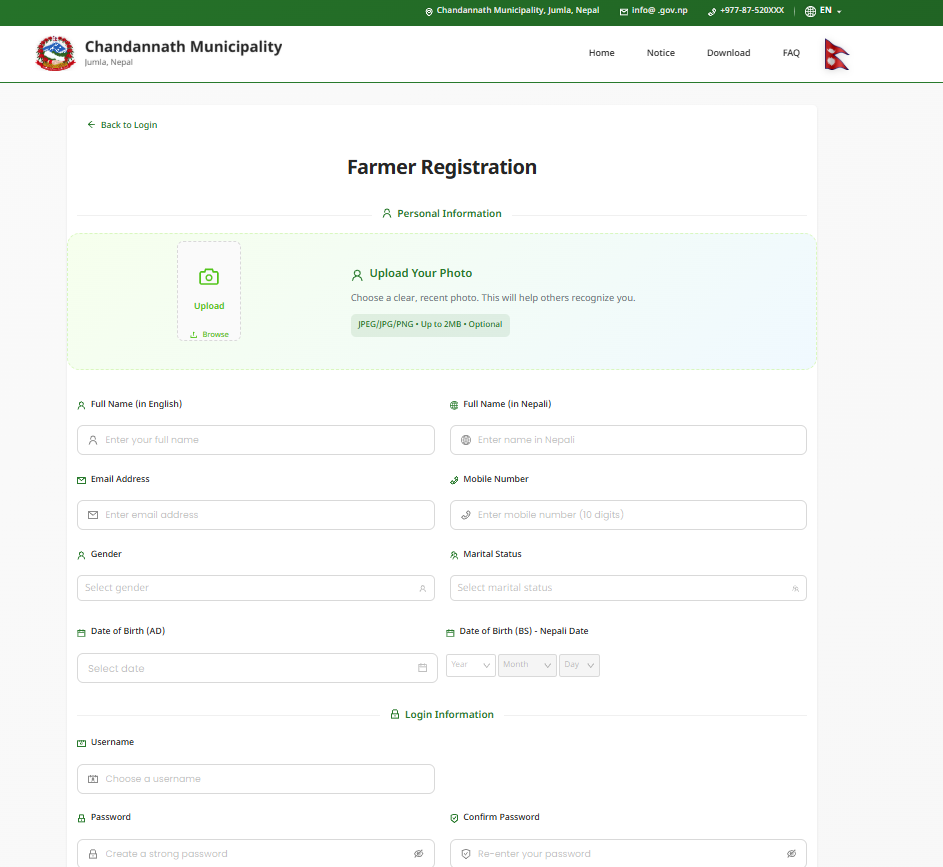
\includegraphics[width=0.85\textwidth]{farmer_form.png}
\caption{Farmer Registration Form with Address Hierarchy}
\label{fig:farmer_form}
\end{figure}

\subsection{Land Plot Module with Leaflet Map}

The Land Plot module integrates \texttt{react-leaflet} for interactive map-based land
management. Field officers draw polygon boundaries directly on the map to define plot
areas, which are stored as GeoJSON coordinates via the API. The map view renders all
registered plots color-coded by land type (irrigated, rain-fed, upland), providing a
ward-level geographic overview. All GeoJSON upload and retrieval endpoints were
tested in Postman before integration.

\begin{figure}[H]
\centering
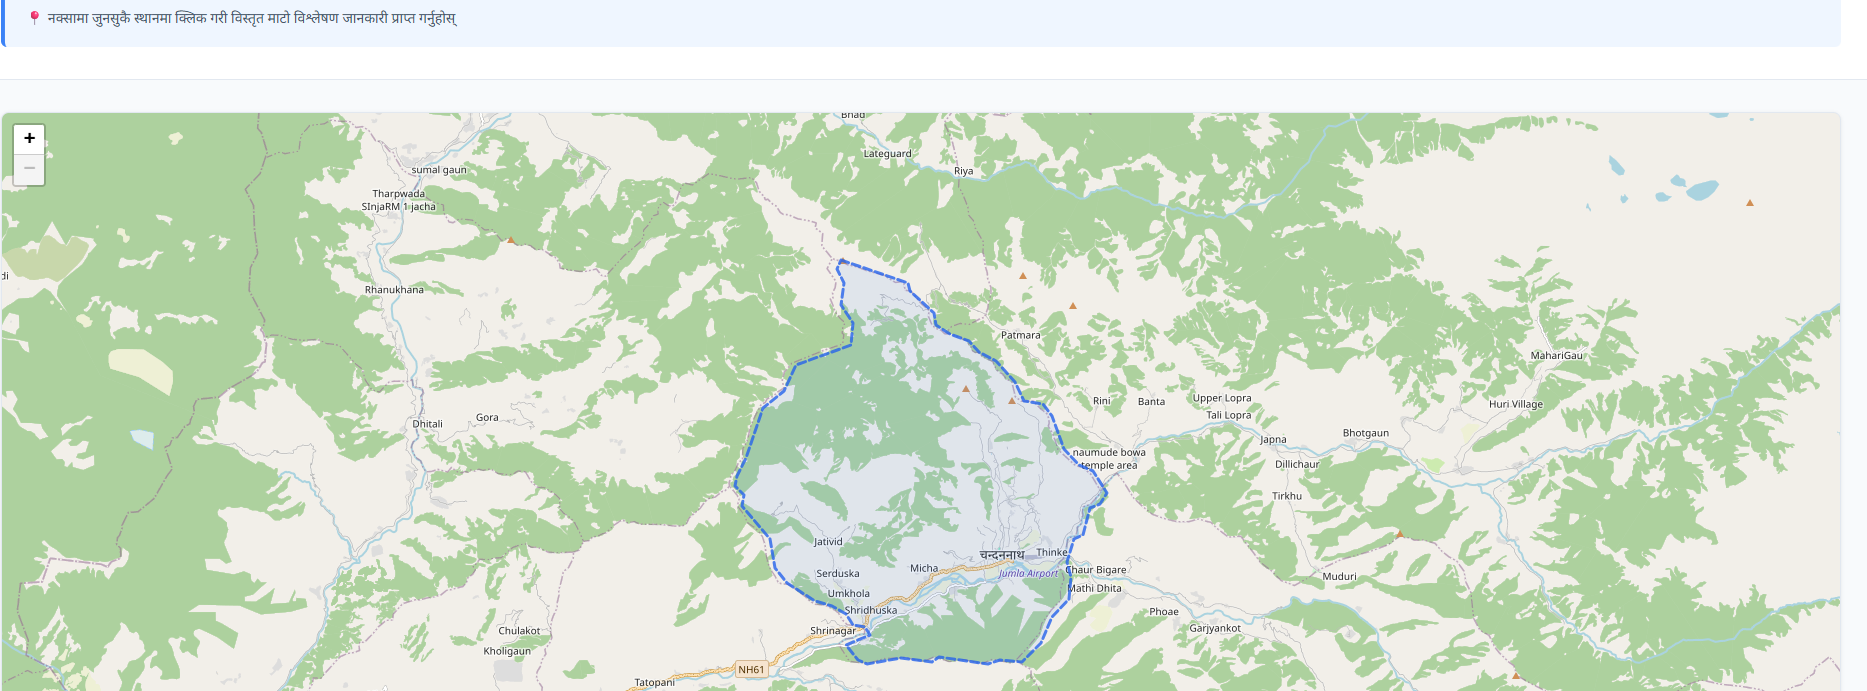
\includegraphics[width=0.85\textwidth]{land_map.png}
\caption{Land Plot Module with react-leaflet Map and Polygon Drawing}
\label{fig:land_map}
\end{figure}

\subsection{Subsidy, Production, Energy, and Financial Modules}

Each of these modules follows a consistent Ant Design table-modal CRUD pattern.
A searchable, filterable, paginated list is the primary view. Creating or editing a record
opens an Ant Design Modal with a validated Form. All module APIs were pre-tested in
Postman. The subsidy module additionally supports dynamic form fields that adapt based
on the selected subsidy type, and implements the multi-municipality configuration pattern
so the same codebase serves all four supported municipalities.

\subsection{Household Survey Module}

The Household Survey module allows department officers to record household-level agricultural
data. Form fields are dynamically generated based on the selected survey template type,
fetched from the backend. Completed surveys are displayed in a searchable list filterable
by ward and date range, and executive users can export results as CSV for offline analysis.

\subsection{Public-Facing Pages}

A separate unauthenticated section provides citizens access to: a \textbf{Notice Board}
with official agricultural notices and pagination; a \textbf{Download Center} for
downloadable guidelines and forms; a bilingual \textbf{FAQ accordion}; a
\textbf{Weather Widget} via open weather API integration; and a \textbf{Soil Analysis}
page fetching results from the NARC API. All public API endpoints were tested in
Postman prior to integration.

\subsection{Deploying the Frontend to Government Cloud Using WinSCP and PuTTY}

The final phase of the internship involved deploying the production-ready AMS frontend
to the government cloud server running Ubuntu 22.04 LTS. The production bundle was
first generated locally using the Vite build command, producing an optimized
\texttt{dist/} directory. WinSCP was then used to securely transfer the \texttt{dist/}
contents to the server web root via SFTP. A PuTTY SSH session was subsequently
opened to configure Nginx as the static file server, enable the site configuration,
set correct file permissions, and reload the service. The critical \texttt{try\_files}
directive in the Nginx server block ensures React Router's client-side routing functions
correctly on the live server. The deployment was verified by confirming the login page
loaded at the production URL and all API calls reached the Spring Boot backend
successfully.

\begin{figure}[H]
\centering
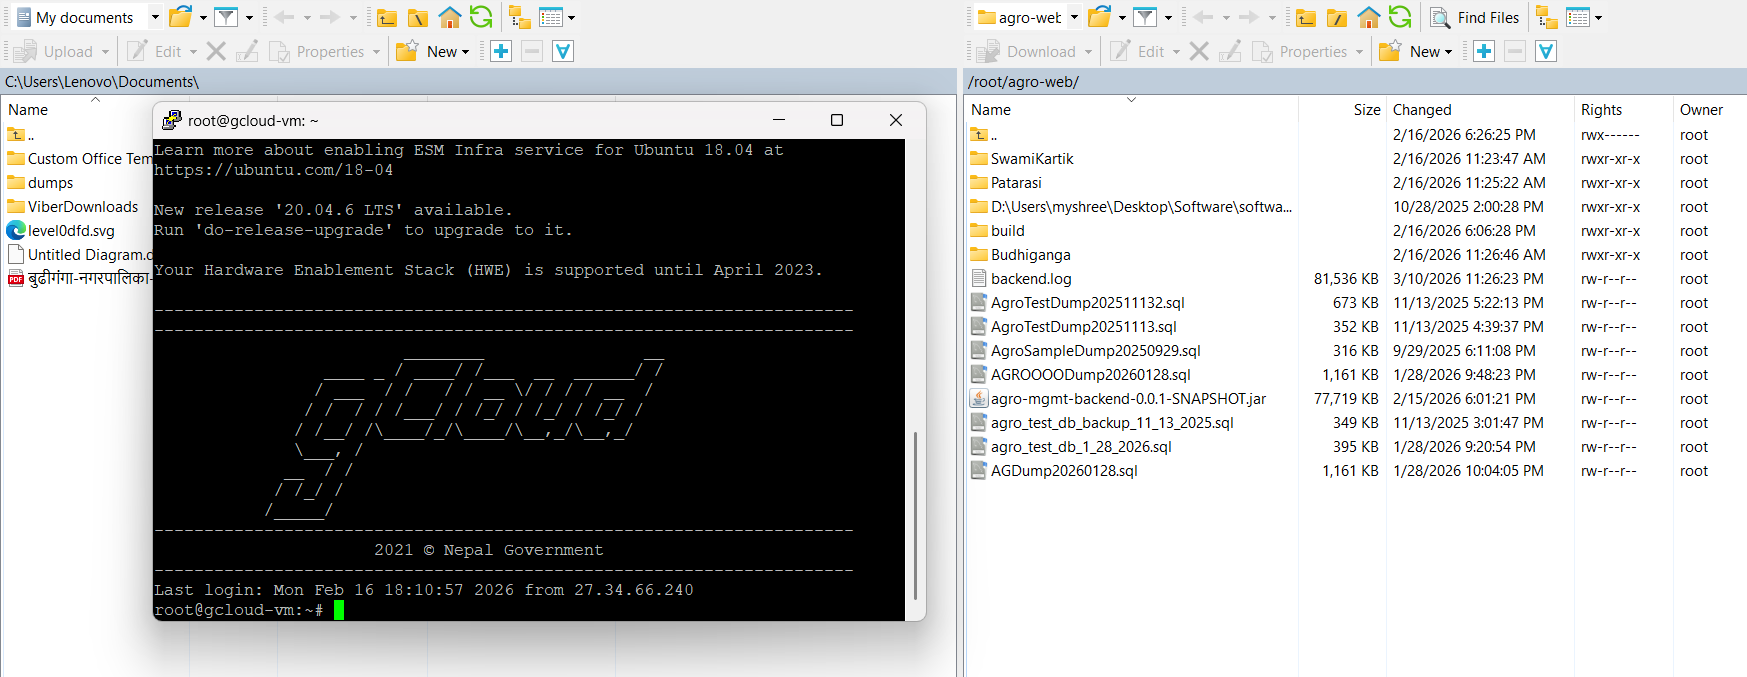
\includegraphics[width=0.85\textwidth]{winscp_upload.png}
\caption{WinSCP File Transfer --- Uploading the Production Build to the Government Server}
\label{fig:winscp}
\end{figure}

\subsection{Performance Optimization}

The final phase focused on performance optimization to reduce unnecessary re-renders, resolving build cache issues, and completing cross-browser testing on Chrome, Firefox, and Edge.

% ════════════════════════════════════════════════════════════════════════════
%  CHAPTER 4: CONCLUSIONS AND LEARNING OUTCOMES
% ════════════════════════════════════════════════════════════════════════════
\chapter{Conclusions and Learning Outcomes}

\section{Conclusions}

The Agriculture Management System developed during this internship successfully
addresses the core challenge facing Nepal's municipal agricultural offices: the absence
of a unified, secure, and locally adapted digital platform for managing farmer data,
land records, subsidies, production statistics, and household surveys across multiple
municipalities.

The system demonstrates that a React.js and TypeScript frontend, built with Ant Design
components and integrated with a Java Spring Boot REST API via JWT-secured Axios
requests, can effectively serve the diverse and demanding requirements of Nepal's
government IT sector. The bilingual interface with runtime Nepali/English toggling and
the cascading Nepal administrative address hierarchy ensure that the platform is genuinely
usable by municipal staff working in Nepali-language environments, directly resolving
one of the most persistent barriers to digital adoption in Nepal's local government sector.

The role-based access control architecture, enforced at both the route and UI rendering
levels for the five roles — Superadmin, Executive, Revenue, Department, and Farmer —
ensures that data security and departmental boundaries are maintained within a single
shared platform. The land plot module with Leaflet-based polygon drawing provides
municipalities with spatial land data management capabilities that were previously
unavailable in paper-based systems, enabling more accurate subsidy targeting and
land ownership verification.

The systematic Postman-first API testing workflow adopted throughout development
proved effective in detecting integration issues early and establishing clear API
contracts between the frontend and backend teams. The successful production deployment
to a government cloud server via WinSCP and Nginx configuration confirms that the
system is ready for live municipal use. Overall, the AMS represents a significant step
toward digital agricultural governance for the municipalities of Chandannath,
Swamikartik, Patarasi, and Budhiganga, with an architecture designed to scale to
additional municipalities with minimal configuration changes.

\section{Learning Outcomes}

\begin{enumerate}[label=\alph*)]

  \item \textbf{React.js and TypeScript:}
  Built production-grade components, custom hooks, and Context API state management
  with strict type safety, improving long-term code reliability and team collaboration.

  \item \textbf{API Integration and Testing with Postman:}
  Developed the discipline of testing every API endpoint before frontend integration,
  creating organized Postman collections with environment variables, auth headers,
  and error-scenario validation. This ensured clean, predictable API contracts.

  \item \textbf{JWT Authentication and Axios Interceptors:}
  Implemented centralized authentication with automatic token attachment, refresh
  handling, and session invalidation on expiry across all modules.

  \item \textbf{Role-Based Access Control (RBAC):}
  Applied RBAC at both the route level (React Router private routes) and UI level
  (conditional rendering of menus and action buttons per role), creating a secure
  and intuitive multi-role user experience.

  \item \textbf{UI/UX Design with Ant Design:}
  Gained proficiency in Ant Design's enterprise component ecosystem, building
  consistent, accessible, and responsive interfaces with clear visual feedback
  for loading, success, and error states across all modules.

  \item \textbf{Nepal-Specific Localization:}
  Acquired specialized skills in Devanagari bilingual context design and cascading
  Nepal address hierarchy --- critical competencies for Nepal's government IT market.

  \item \textbf{GIS and Leaflet.js Integration:}
  Implemented interactive maps with polygon drawing, GeoJSON storage, and
  layer-based land type visualization for agricultural geographic data.

  \item \textbf{Frontend Deployment with WinSCP and PuTTY:}
  Gained hands-on experience building production Vite bundles and deploying them
  to Linux-based government cloud servers using WinSCP for secure file transfer
  and PuTTY for remote SSH administration and Nginx configuration.

  \item \textbf{Agile Development and Professional Practices:}
  Participated in full sprint cycles, daily stand-ups, code reviews, and retrospectives.
  Learned to estimate tasks, manage priorities, and deliver features incrementally
  in a professional team environment.

\end{enumerate}

% ─────────────────────────────────────────────────────────────────────────────
%  REFERENCES
% ─────────────────────────────────────────────────────────────────────────────
\newpage
\renewcommand{\bibname}{REFERENCES}
\bibliographystyle{apacite}
\begin{thebibliography}{}

\bibitem[Adhikari et al.(2022)]{adhikari2022}
Adhikari, P., Shrestha, B., \& Karki, R. (2022). Localization challenges in developing government web applications for Nepal: Bikram Sambat calendar integration. \textit{Journal of IT Nepal}, 5(1), 12--24.

\bibitem[Banks \& Porcello(2020)]{banks2020}
Banks, A., \& Porcello, E. (2020). \textit{Learning React: Modern patterns for developing React apps} (2nd ed.). O'Reilly Media.

\bibitem[Cherny(2019)]{cherny2019}
Cherny, B. (2019). \textit{Programming TypeScript: Making your JavaScript applications scale}. O'Reilly Media.

\bibitem[CS Sewa(2024)]{cssewa2024}
CS Sewa Pvt. Ltd. (2024). \textit{About us}. Retrieved March 11, 2026, from https://www.cssewa.com.np

\bibitem[FAO(2021)]{fao2021}
Food and Agriculture Organization of the United Nations. (2021). \textit{Digital agriculture: Pathways to transforming agri-food systems}. FAO. https://doi.org/10.4060/cb4662en

\bibitem[Ferraiolo et al.(2001)]{ferraiolo2001}
Ferraiolo, D. F., Sandhu, R., Gavrila, S., Kuhn, D. R., \& Chandramouli, R. (2001). Proposed NIST standard for role-based access control. \textit{ACM Transactions on Information and System Security}, 4(3), 224--274. https://doi.org/10.1145/501978.501980

\bibitem[Jones et al.(2015)]{jones2015}
Jones, M., Bradley, J., \& Sakimura, N. (2015). \textit{JSON Web Token (JWT)} (RFC 7519). Internet Engineering Task Force. https://doi.org/10.17487/RFC7519

\bibitem[Sohan et al.(2017)]{sohan2017}
Sohan, S. M., Maurer, F., Anslow, C., \& Robillard, M. P. (2017). A study of the effectiveness of usage examples in REST API documentation. In \textit{Proceedings of the 2017 IEEE Symposium on Visual Languages and Human-Centric Computing (VL/HCC)} (pp. 53--61). IEEE. https://doi.org/10.1109/VLHCC.2017.8103455

\end{thebibliography}

% ─────────────────────────────────────────────────────────────────────────────
%  ANNEX: SCREENSHOTS
% \newpage
\chapter*{Annex: (Screenshots)}
\addcontentsline{toc}{chapter}{Annex: Screenshots}

\begin{figure}[H]
\centering
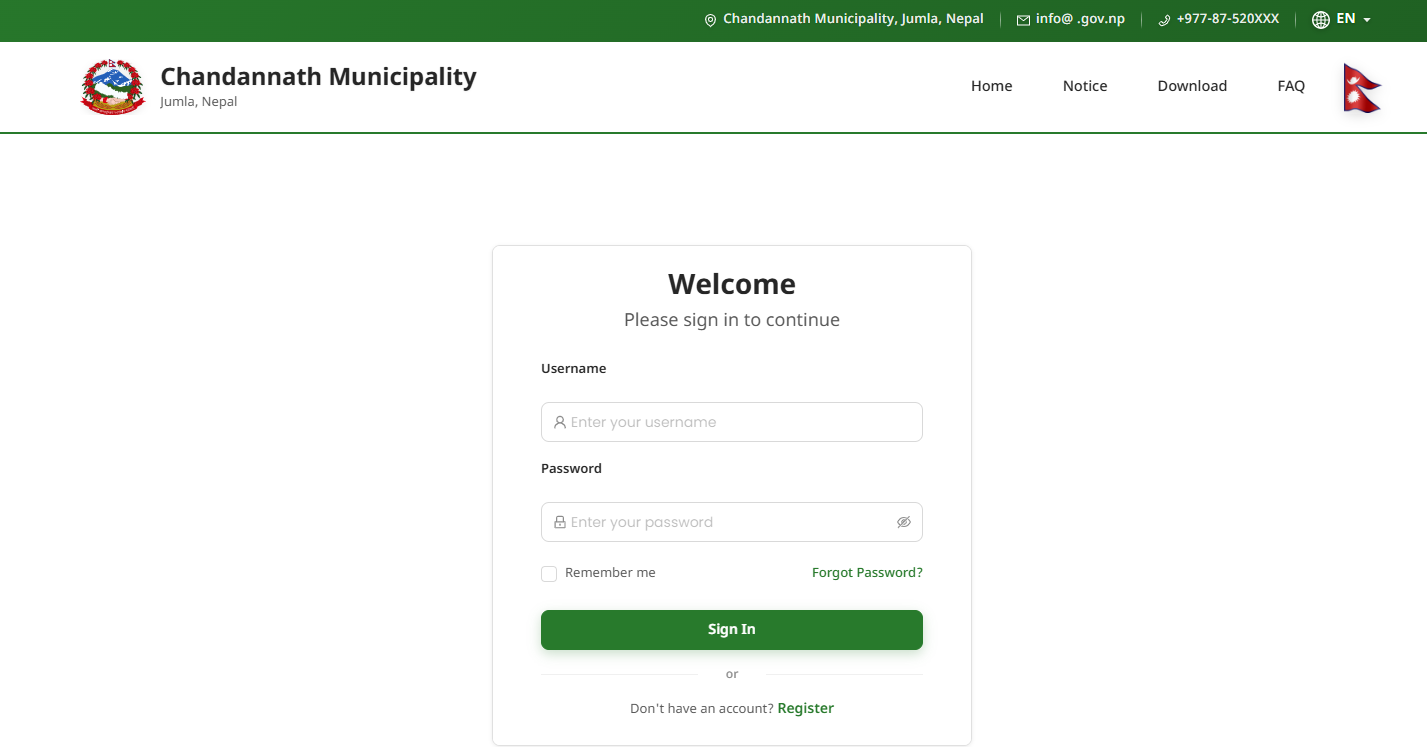
\includegraphics[width=0.85\textwidth]{login_page.png}
\caption*{Login Page of the Agriculture Management System}
\end{figure}

\begin{figure}[H]
\centering
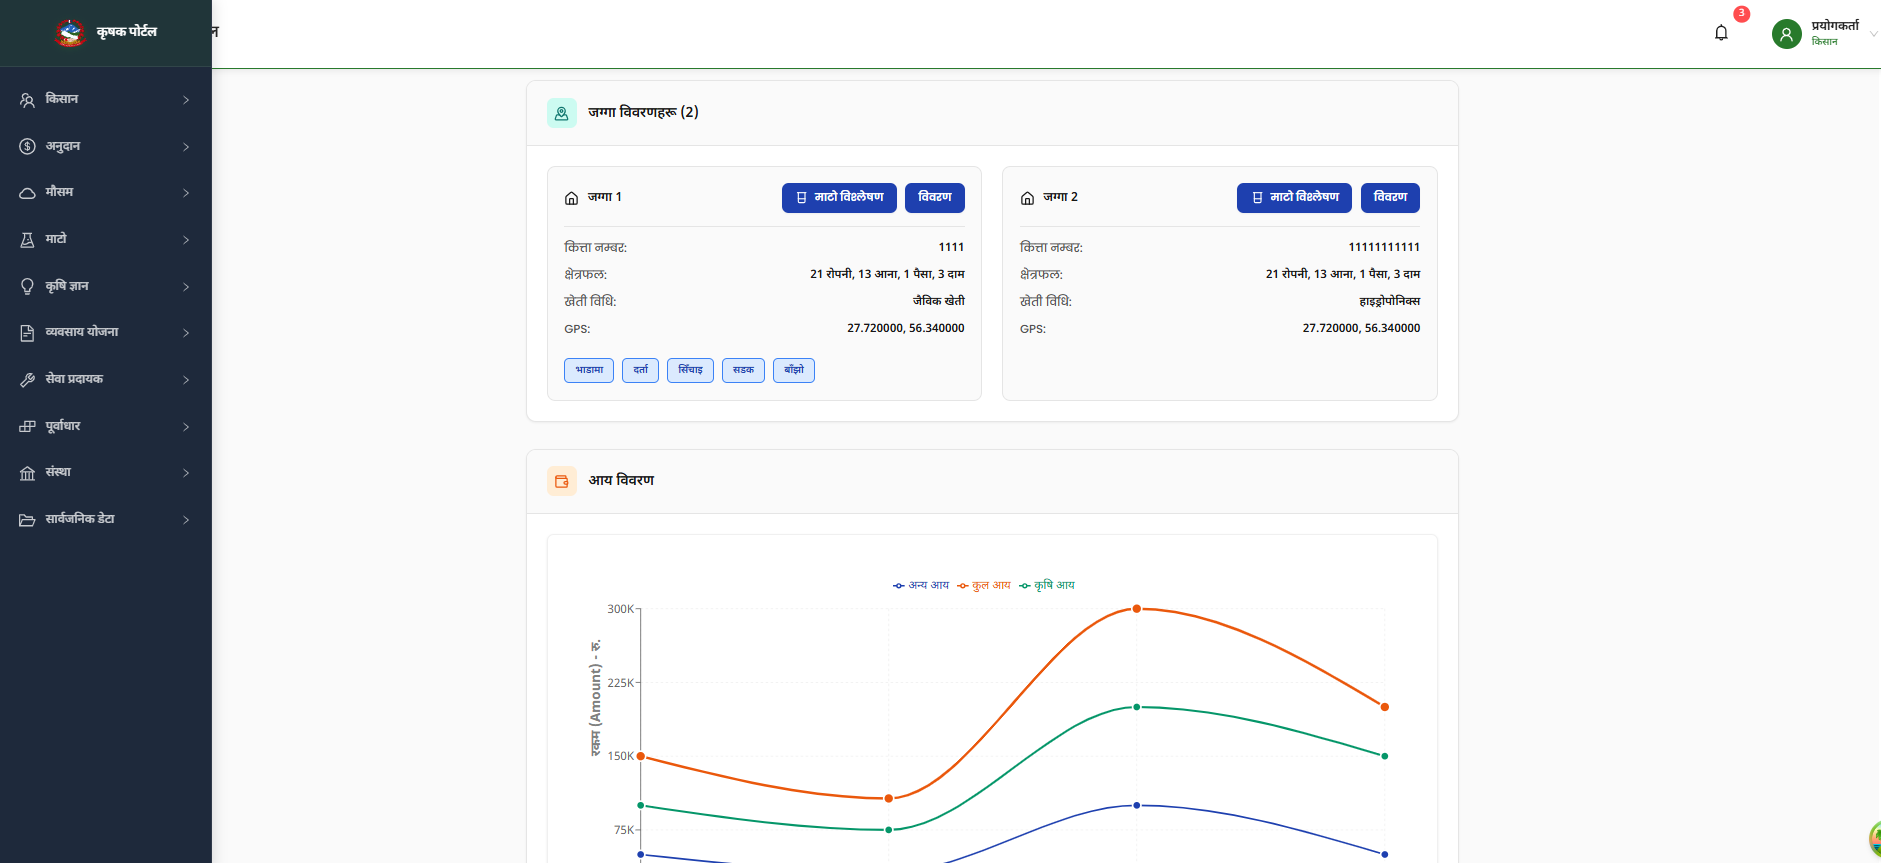
\includegraphics[width=0.85\textwidth]{farmer.png}
\caption*{Farmer Dashboard}
\end{figure}

\begin{figure}[H]
\centering
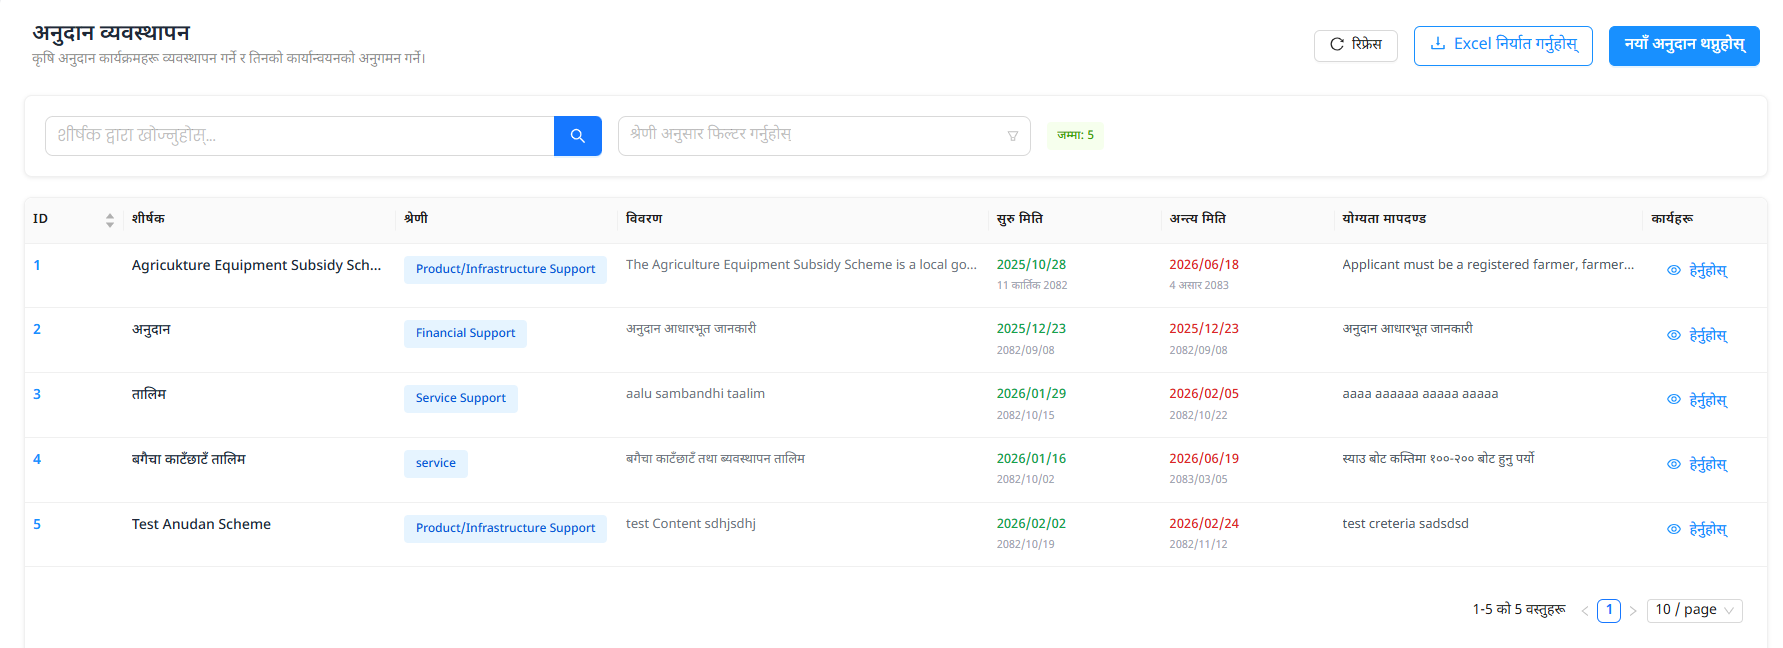
\includegraphics[width=0.85\textwidth]{subsidy_module.png}
\caption*{Subsidy Program Management Module}
\end{figure}

\begin{figure}[H]
\centering
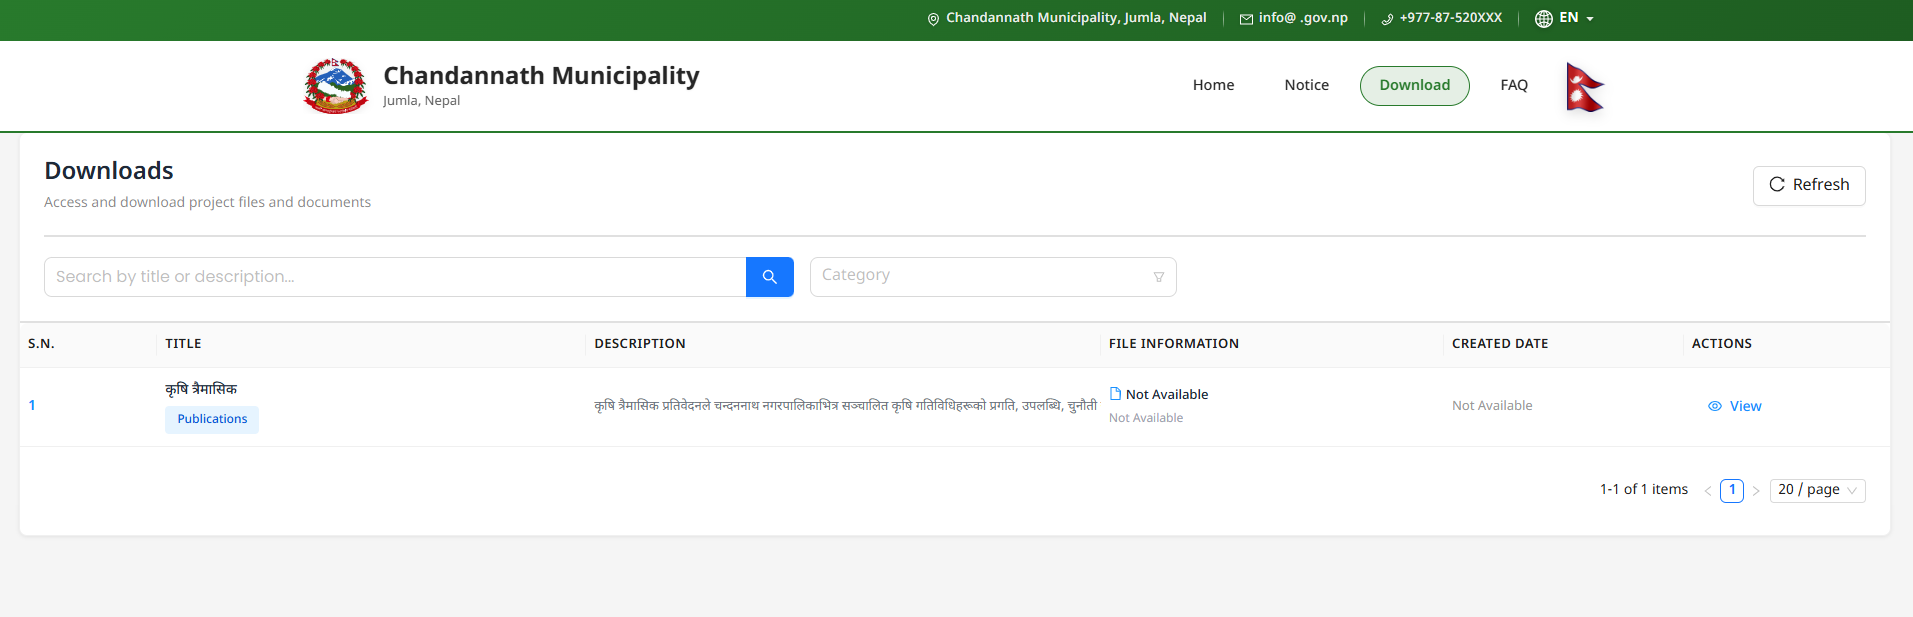
\includegraphics[width=0.85\textwidth]{public_pages.png}
\caption*{Public-Facing Download Center}
\end{figure}

\begin{figure}[H]
\centering
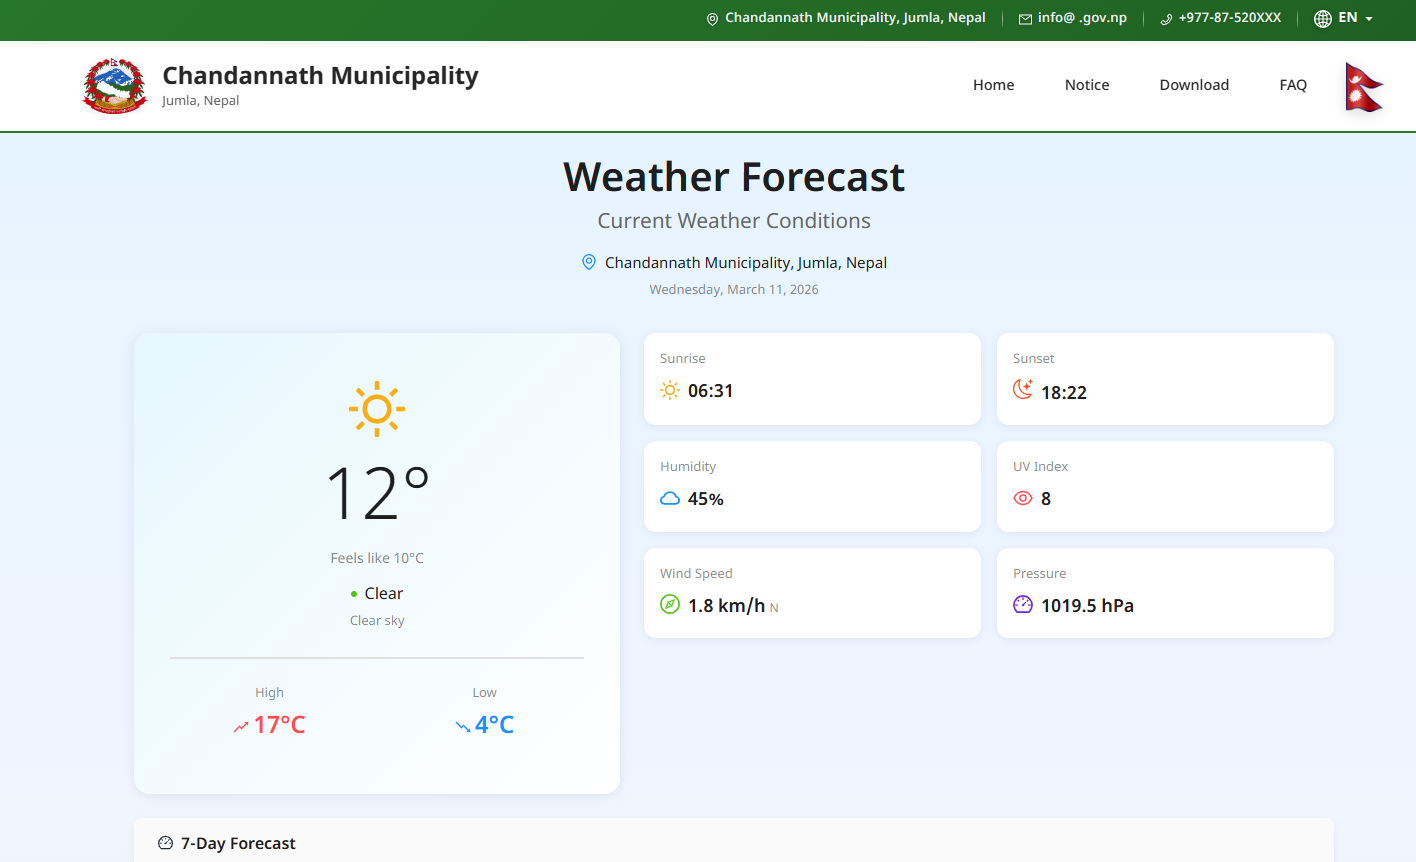
\includegraphics[width=0.85\textwidth]{weather.png}
\caption*{Weather Dashboard --- Weather Information Page}
\end{figure}

\end{document}